\documentclass[titlepage,oneside]{article}

\usepackage{todonotes}
\usepackage{graphicx}
\usepackage{subcaption}
\graphicspath{ {./images/} }
\usepackage{hyperref}
\usepackage{pdfpages}
\usepackage{cite}
\usepackage{url}
\usepackage{multirow}
\usepackage{booktabs}


\newcommand{\figref}[1]{Figure ~\ref{fig:#1}}

\title{An Analysis of Best Practices in Traffic Calming}

\author{
	Jake Hermle\\ \emph{Civil Engineering} \and
	Nakul Joshi\\ \emph{Computer Engineering} \and
	John Lally\\ \emph{Mechanical Engineering}\and
	Christine Noh\\ \emph{International Relations}
}

\date{6\textsuperscript{th} December, 2013}

%ADD LETTERS

\begin{document}
\listoftodos

\newpage
\todo[inline]{Christine: Letter to CHC}

\maketitle

\begin{abstract}
\todo[inline]{Christine: Write the abstract}
In order to improve mobility and safety in Los Angeles, we have looked upon eight distinctive traffic-calming practices. These include chokers, curb radius, raised crosswalks, curb extensions, textured pavements, dignified zones, traffic circles, and midblock crossings. We will go in detail for each of these techniques and in the end, discuss which one would be the better alternative for Los Angeles specifically. 
\end{abstract}


\tableofcontents
\newpage
\listoffigures
\newpage
\listoftables
\newpage



\section{Introduction and Background}

Community Health Councils (CHC) is producing a report for the City of Los Angeles that recommends and details guidelines for complete streets design to be included in the Mobility Element of the city’s General Plan. This CHC report will be describing various best practices that can be implemented so that LA streets better adhere to the principles of complete streets. The following report details eight specific best practices that CHC may implement in their report to the City of Los Angeles. For each best practice, a general description is provided, as well as a discussion of its impact and cost. Additionally, each practice was evaluated based on its cost, impact, and ease of implementation to determine whether it is worth recommending as a design guideline in the Mobility Element. A usability index was created to more quantitatively evaluate these practices, and allowed for better comparison between them. In addition to complete street design, this report is also mindful of CHC’s overarching goals of improving health in South LA.

\todo[inline]{John: Finish this section}

\newpage

\section{Best Practices}

	\subsection{Chokers}
	Chokers are curb extensions at midblock locations that narrow a street by ultimately creating wider sidewalks. They are also known as safe crosses when marked as crosswalks. Chokers can be made by widening one side of the curb or by bringing both curbs in, giving it the “pinch point” along the street (See \figref{choker}). The main purpose of chokers is to decrease speed of incoming vehicles at a mid-point along the streets, create a seamless transition between a commercial and a residential area, and to narrow exceedingly wide intersections \cite{walking-info-chokers}.

\begin{figure}[h]
\centering
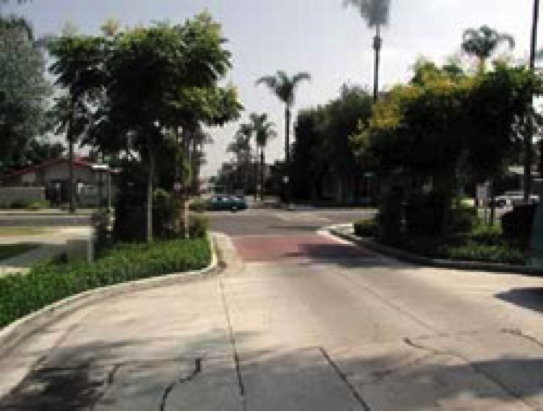
\includegraphics[scale=1]{choker.png}
\caption[Choker]{This choker requires drivers to yield upon entering}\label{fig:choker}
\end{figure}

Two-lane chokers (See \figref{two-lane-choker}) leave two lanes in the street cross section narrower than the width of a normal cross section, while one-lane chokers narrow the width to allow travel in only one direction at a time. These chokers are effective for areas with substantial speed problems and streets with minimum or no parking on-site.

\begin{figure}
\centering
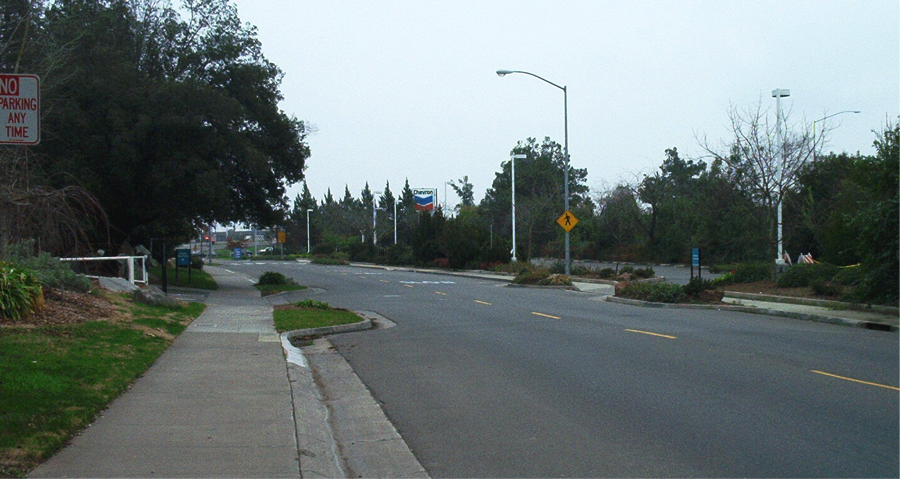
\includegraphics[scale=1]{two-lane-choker.png}
\caption{Two-Lane Chokers}\label{fig:two-lane-choker}
\end{figure}

\subsubsection{Advantages and Disadvantages}

The various advantages of chokers are:\begin{itemize}
\item ability to reduce both speed and volume significantly
\item easily negotiable by large vehicles (for example, fire trucks)
\item improving aesthetic value when well designed
\end{itemize}

The disadvantages include:\begin{itemize}
\item Eliminates on-street parking
\item Requires bicyclists to briefly merge with vehicular traffic
\item Absence of vertical or horizontal deflation limiting the effect of chokers on vehicle speed.
\end{itemize}

\subsubsection{Effectiveness}

Chokers can ultimately increase the visibility of pedestrians as well as to reduce pedestrian crossing width, while the speed of vehicles is reduced by 4 percent on average for two-lane chokers and 14 percent on average for one-lane chokers \cite{ite}. Also since chokers work well with speed humps, speed tables, and raised intersections, (See \figref{speed-hump}) it can be created in many sites with no extreme difficulty.

\begin{figure}
\centering
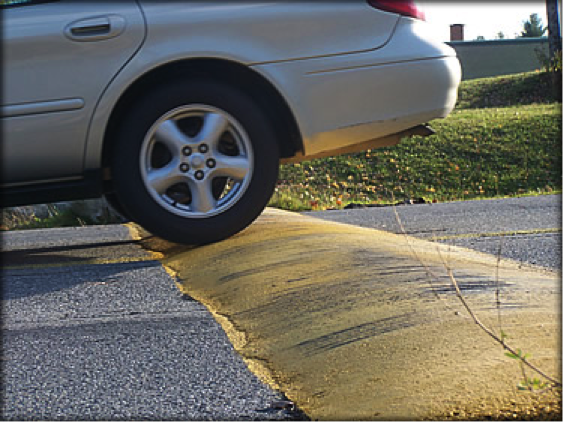
\includegraphics[scale=1]{speed-hump.png}
\caption{Speed Hump}\label{fig:speed-hump}
\end{figure}

\subsubsection{Cost and Considerations}

Factors to consider when creating chokers are to consult with the local fire and sanitation department before setting minimum width and to double check to make sure that the bicyclist safety and mobility are not diminished. Also when reducing two-lane street to one lane, the width of the travel way should not be wide enough for 2 cars to pass at the same time. This equals to the travel way not being wider than 4.9 meter, or 16 to 17 feet; by doing so, the effectiveness of the chocker is maximized \cite{walking-info-chokers}. The cost to create chokers varies depending on the site and landscape but most are along the lines of \$5,000 to \$20,000 (drainage representing a significant amount).
	
	\subsection{Curb Radius}
	Curb radius is a traffic calming technique in which the grid of intersecting streets is reshaped and the radius of the curb is significantly reduced. As you can see in \figref{large-radius}, a large curb radius will enable vehicles to go around corners faster while in \figref{small-radius}, a smaller curb radius will slow vehicles down when turning into the corner.

\begin{figure}[h]
\centering
\begin{subfigure}[b]{0.4\textwidth}
	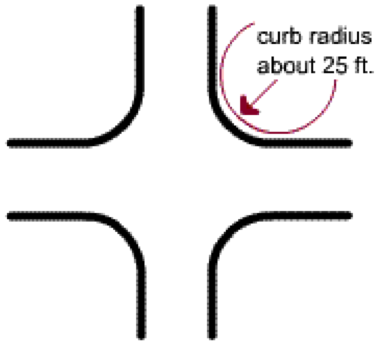
\includegraphics[width=\textwidth]{large-radius.png}
	\caption{Large Curb Radius}\label{fig:large-radius}
\end{subfigure}
\begin{subfigure}[b]{0.4\textwidth}
	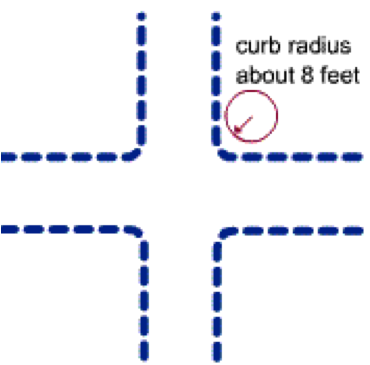
\includegraphics[width=\textwidth]{small-radius.png}
	\caption{Small Curb Radius}\label{fig:small-radius}
\end{subfigure}
\end{figure}

        The purpose of curb radii is to slow vehicles down by enabling them to make smaller turns, which ultimately reduces the risk of pedestrians being struck by vehicles when turning into a corner. Also, small curve radii can create safer intersections, improve the visibility between drivers and pedestrians, and lead to improved signal timing. By reducing the curb radii, not only will it slow down vehicles when turning, but it will also shorten the distance and time it takes for pedestrians to cross the street by nearly half of what it used to be (See Table ~\ref{table:cross-time-vs-radius} and Figures ~\ref{fig:radius-change} and ~\ref{fig:cross-time-vs-radius}).
        
\begin{figure}[h]
\centering
	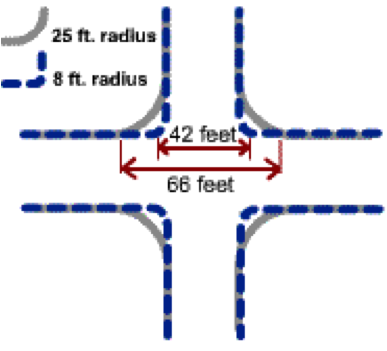
\includegraphics[scale=1]{radius-change.png}
	\caption[Effect of changing curb radius]{Change in Distance from 25ft. Radius to 8ft. Radius}\label{fig:radius-change}
\end{figure}

\begin{table}[h]
\centering
    \begin{tabular}{cc}
    Curb Radius (feet) & Average crossing time (seconds) \\ \hline
    10                 & \phantom{0}7.9                             \\
    15                 & \phantom{0}9.8                             \\
    25                 & 14.1                            \\
    \end{tabular}
\end{table}

\begin{figure}[h]
\centering
	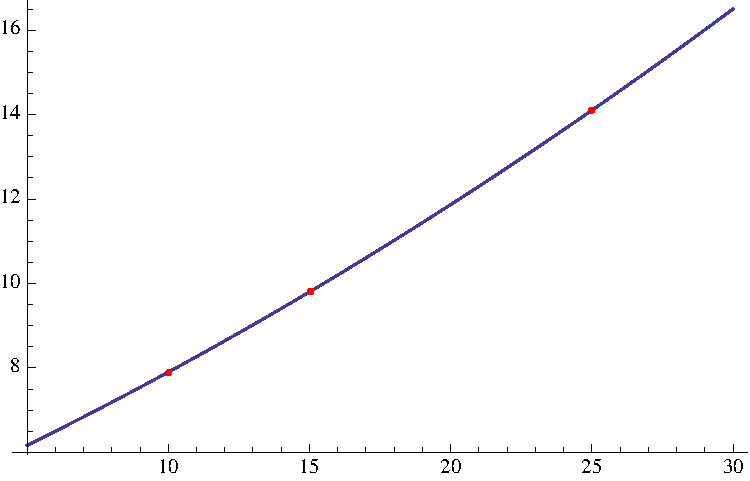
\includegraphics[scale=0.5]{cross-time-vs-radius.pdf}
	\caption[Plot of crossing times against curve radii]{A plot of the data from Table ~\ref{table:cross-time-vs-radius}}\label{fig:cross-time-vs-radius}
\end{figure}

        When streets have a large curb radius, motorists can make turns at relatively high speeds that decrease pedestrian safety. By contrast, 90-degree intersections and corners with tight curb radii tend to slow motorists down and therefore increase pedestrian safety. Motorists turning right at high speed can cut off bicyclists/pedestrians traveling straight on the arterial street. In addition, pedestrians crossing the residential street adjacent to the arterial may not expect high-speed turning traffic, or they may have their backs facing the turning cars as you can see in ~\ref{fig:back-against-car}

\begin{figure}
\centering
	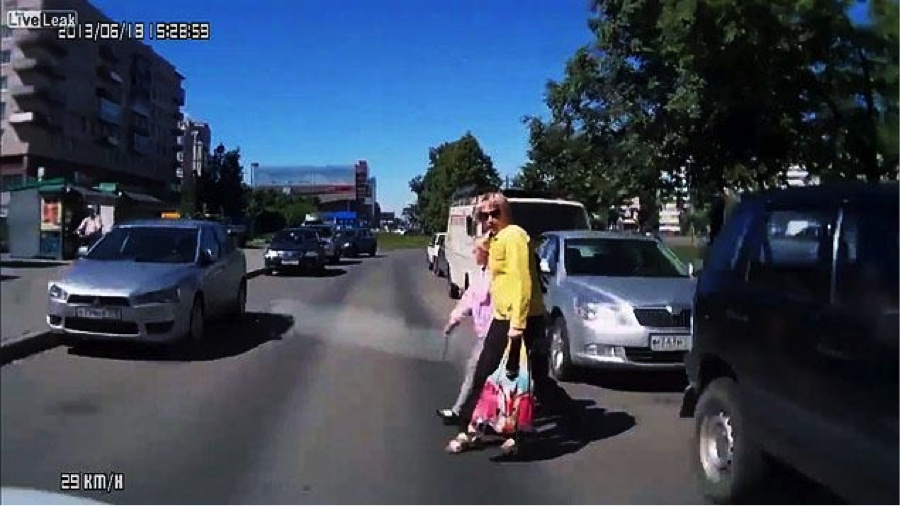
\includegraphics[width=0.5\textwidth]{back-against-car.png}
	\caption{Pedestrian Facing Back Against the Car}\label{fig:back-against-car}
\end{figure}

The cost of reconstructing tighter turning radii is in between \$5,000 to \$40,000 per corner depending on the site locations/conditions. When considering curb radii, it is important to note that in order for it to be effective, the design should meet the needs of the design vehicles with consideration for nearby land uses and prevalence of roadway users. So if there are high volumes of large vehicles making turns in a given location, a poorly designed curb radius could potentially cause the vehicles to drive over the curb and onto the sidewalk endangering pedestrians. In addition, you should always accommodate emergency vehicles, as well as school buses, and public maintenance vehicles when designing curb radii\cite{walking-info-curb}.


There is no magic number for the appropriate curb radius because it differs case by case depending on where it is located (See \figref{location-depend}). The length of the curb radius that should be used wherever possible is 5 to 10 feet, whereas an effective radius for urban streets with high volumes of pedestrians is 15 to 20 ft. For arterial streets with a substantial volume of turning buses/trucks, an appropriate effective curb radius is about 25 to 30 ft.; and the maximum desired effective curb radius is typically 35 feet for large vehicles \cite{walking-info-curb}.

\begin{figure}
\centering
	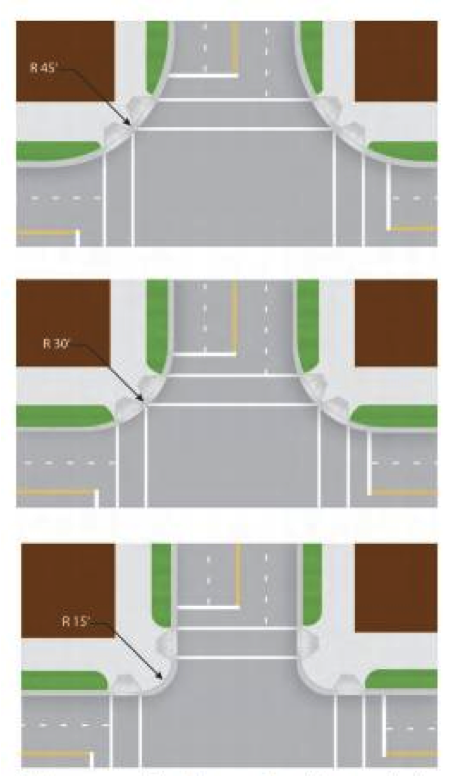
\includegraphics[scale=0.5]{location-depend.png}
	\caption{Different Curb Radii Depending on the Location}\label{fig:location-depend}
\end{figure}
	
\newpage

	\subsection{Raised Crosswalks}
	A raised crosswalk (\figref{xwalk}) is a designated street crossing that simulatneously acts as a speed hump by bringing the level of the roadway to that of the sidewalk.

\begin{figure}[h]
	\centering
	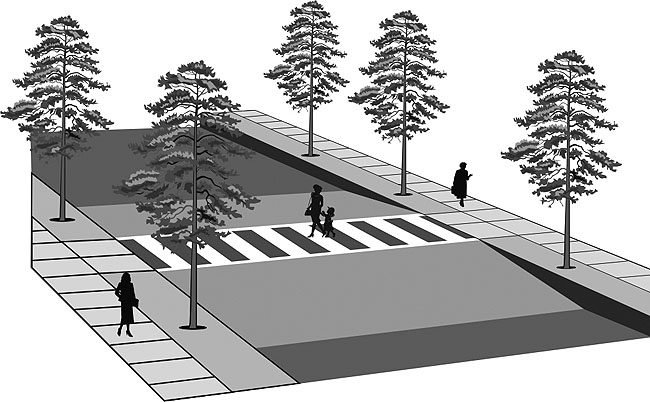
\includegraphics[width=0.7\textwidth]{xwalk.jpg}
	\caption[A raised crosswalk]{A raised crosswalk\cite{kimley-xwalk}}\label{fig:xwalk}
\end{figure}

\subsubsection{Advantages and Disadvantages}

The advantages of such a traffic calming measure include:\begin{itemize}
	\item Forces traffic to slow down, improving pedestrian safety.
	\item Draws attention to the pedestrian, especially when combined with signage and markings.
	\item Makes crossing the street easier for those on wheelchairs.
\end{itemize}

The drawbacks are:\begin{itemize}
	\item The textured materials used tend to be expensive.
	\item Not suitable for emergency or bus routes.
	\item Drainage, especially in snowy or rainy areas, requires additional management.
\end{itemize}

\subsubsection{Effectiveness}

Raised crosswalks are an effective traffic calming technique in that they can reduce vehicular speed (See Table ~\ref{table:xwalk-speed-reduction}). Further, they have also been shown effective at encouraging pedestrians to use the crosswalk instead of crossing the road elsewhere. One study \cite{pedsafe-xwalks} found that raising the crosswalk increased the percentage of pedestrians using it from 11.5\% to 38.3\%. 

% Please remember to add \use{multirow} to your document preamble in order to suppor multirow cells
% Booktabs require to add \usepackage{booktabs} to your document preamble
\begin{table}[h]
\begin{tabular}{@{}lrrr@{}}
\toprule
\multirow{2}{*}{City and Measure}    & \multicolumn{2}{l}{50th percentile speed (km/h)} & \multirow{2}{*}{Speed reduction (km/hr)} \\ \cmidrule(lr){2-3}
      & Treatment Site           & Control Site          &                  \\ \midrule
\begin{tabular}[l]{@{}l@{}}Durham, NC – Research Drive\\ \textit{Raised crosswalk}\end{tabular}                    & 33.3                     & 39.8                  & 6.5                                      \\
\begin{tabular}[l]{@{}l@{}}Durham, NC – Towerview Drive\\ \textit{Raised crosswalk, overhead flasher}\end{tabular} & 18.5                     & 38.4                  & 19.3                                     \\
\begin{tabular}[l]{@{}l@{}}Montgomery County, MD\\ \textit{Raised Crosswalk}\end{tabular}                          & 34.6                     & 38.6                  & 4.0                                   
\\ \bottomrule
\end{tabular}
\caption{Speed reduction due to raised crosswalks}
\end{table}

According to PEDSAFE \cite{pedsafe-xwalks}, raised crosswalks can mitigate dart-and-dash type incidents in which the driver was unable to see the pedestrian until just before impact. They also prevent vehicles from `trapping' pedestrians. Raised crosswalks are best used in areas of low-volume, low-speed traffic where safety of pedestrians takes a priority, such as residential areas and near schools. As a side benefit, they make crossings much easier for the elderly, the disabled, and the young in these areas.

\subsubsection{Cost and Considerations}

The cost of such a crosswalk varies from \$,2000 to \$15,000, with typical cost estimate for one unit being \$4000\cite{traffic-calming-xwalks}. However, this might be significantly increased if a drainage system has to be added.

\begin{figure}[!htbp]
\centering
\begin{subfigure}[t]{0.45\textwidth}
	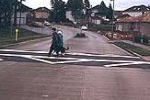
\includegraphics[width=0.9\textwidth]{xwalk1}
	\subcaption{Asphalt and highly-visible paint.}
\end{subfigure}
\begin{subfigure}[t]{0.45\textwidth}
	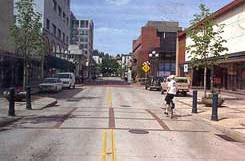
\includegraphics[width=0.9\textwidth]{xwalk2}
	\subcaption{Concrete and brick.}
\end{subfigure}\\
\begin{subfigure}[t]{0.45\textwidth}
	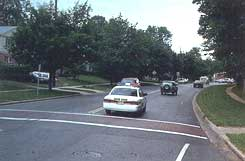
\includegraphics[width=0.9\textwidth]{xwalk3}
	\subcaption{Tapering at the curbs to allow drainage.}
\end{subfigure}
\begin{subfigure}[t]{0.45\textwidth}
	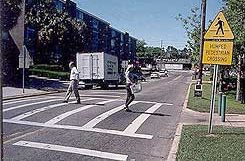
\includegraphics[width=0.9\textwidth]{xwalk4}
	\subcaption{Higher profile crosswalk, almost resembling a speed hump.}
\end{subfigure}
\caption[Various raised crosswalk styles]{Various raised crosswalk styles.\cite{traffic-calming-xwalks}}
\end{figure}

\newpage

\newpage

	\subsection{Curb Extensions}
	A curb extension (\figref{curb-extension}) is an extension of the curb onto the roadway. As a traffic calming measure, they are primarily used to assist pedestrians by reducing crossing distance and slowing traffic down.

\begin{figure}[h]
\centering
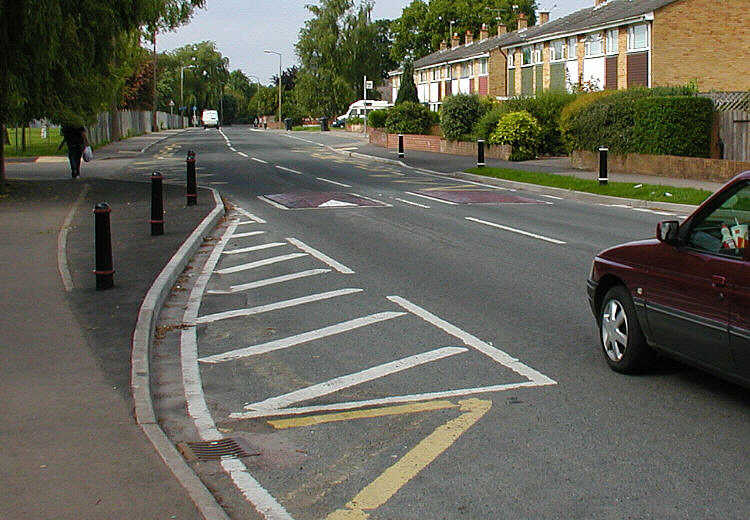
\includegraphics[width= 0.5\textwidth]{curb-extension}
\caption{Curb extension}\label{fig:curb-extension}
\end{figure}

\subsubsection{Advantages and Disadvantages}

Curb extensions are thought to have the following advantages:\begin{itemize}
\item Reduce the time that pedestrians are exposed to traffic.
\item Increase the visibility of pedestrians attempting to cross.
\item Shield parking lanes from oncoming traffic and prevent drivers from using them as right turn lanes.
\end{itemize}

The various drawbacks are:\begin{itemize}
\item They pose a threat to bicyclists, who are forced into a narrowed gap along with traffic.
\item Like raised crosswalks, they complicate drainage since they obstruct the gutter.
\item Reduce the availibility of parking spaces, which can hurt local businesses.
\end{itemize}

\subsubsection{Effectiveness}

One study \cite{randal05} found that curb extensions significantly reduced the number of vehicles pedestrians had to wait for before one yielded. The same study also found minor increases in percents of crossings where a motorist yielded, and of vehicles yielding at advance stop bars. These results are shown in Tables ~\ref{table:vehicles-passed}, \ref{table:motorist-yielded} and \ref{table:motorist-stop-bar}.

\subsubsection{Cost and Considerations}

Curb extensions cost between \$5,000 and \$25,000 per corner\cite{walking-info-enhancements}. As with most sidewalk retrofitting, a large portion of the cost goes to drainage. If it is also necessary to remove a utility pole or other such existing infrastructure element, costs can become much higher.

% Booktabs require to add \usepackage{booktabs} to your document preamble
\begin{table}[!htbp]
\centering
\begin{tabular}{@{}crrrr@{}}
\toprule
\multicolumn{1}{l}{Lane} & \multicolumn{1}{l}{Non-curb extension} & \multicolumn{1}{l}{Curb extension} & \multicolumn{1}{l}{Difference} & \multicolumn{1}{l}{Sample Size} \\ \midrule
Near                     & 2.58                                   & 1.81                               & -42.7 \%                            & 219                             \\
Far                      & 2.36                                   & 1.76                               & -33.9  \%                           & 214                           \\
\bottomrule 
\end{tabular}
\caption{Average number of vehicles passing before a pedestrian-cross. Results found significant by the t-test.}\label{table:vehicles-passed}
\end{table}
% Booktabs require to add \usepackage{booktabs} to your document preamble
\begin{table}[!htbp]
\centering
\begin{tabular}{@{}crrrr@{}}
\toprule
\multicolumn{1}{l}{Lane} & \multicolumn{1}{l}{Non-curb extension} & \multicolumn{1}{l}{Curb extension} & \multicolumn{1}{l}{\% difference} & \multicolumn{1}{l}{Sample Size} \\ \midrule
Near                     & 64.9\%                                 & 66.7\%                             & 2.7\%                             & 234                             \\
Far                      & 58.6\%                                 & 63.4\%                             & 7.7\%                             & 234                            \\
\bottomrule
\end{tabular}
\caption{Percents of pedestrian crossings with yield. The results were found insignificant by the t-test.}\label{table:motorist-yielded}
\end{table}
% Booktabs require to add \usepackage{booktabs} to your document preamble
\begin{table}[!htbp]
\centering
\begin{tabular}{@{}crrrr@{}}
\toprule
\multicolumn{1}{l}{Lane} & \multicolumn{1}{l}{Non-curb extension} & \multicolumn{1}{l}{Curb extension} & \multicolumn{1}{l}{\% difference} & \multicolumn{1}{l}{Sample Size} \\ \midrule
Near                     & 42.6\%                                 & 53.8\%                             & 21.0\%                            & 99                              \\
Far                      & 42.6\%                                 & 51.9\%                             & 18.0\%                            & 99                            \\
\bottomrule 
\end{tabular}
\caption{Percent of vehicles yielding at advance stop bar. The results were found insignificant by the t-test.}\label{table:motorist-stop-bar}
\end{table}
	
\newpage
	\subsection{Textured Pavements}
		\todo[inline]{Jake: Add the textured pavements section}
		Textured and colored pavements refers to the use of varied pavement materials to alter the color or texture of a street surface. This practice can be used as a traffic calming measure or as a way to distinguish special areas of the street.

Changes in pavement texture from normal concrete or asphalt surfaces can cause a change in audible road noise inside the car body. This effect can be utilized to alert drivers to slow down or take notice of potential hazards. Textured or colored pavements can also be used to visually distinguish special areas of the street, such as crosswalks or bike lanes, to make drivers more aware of their location \cite{TP1}.

Altered pavement textures and colors have been found to cause reductions in vehicle speed, though there is limited data available to quantify this \cite{TP3}. This practice can be used in combination with other practices to produce a traffic calming effect, such as raised crosswalks, speed tables, or raised intersections. 

\subsubsection{Materials}

\paragraph{Cobblestones} Cobblestone roads are paved with quarried stone with rounded tops. The advantages of this material are that it will create a significant audible disturbance to drivers and can provide a unique aesthetic appeal; however, cyclists and wheelchair users might find this pavement difficult to navigate. Additionally, the unevenness of the pavement makes it more difficult to remove snow and ice \cite{TP6}.

\begin{figure}[h]
\centering
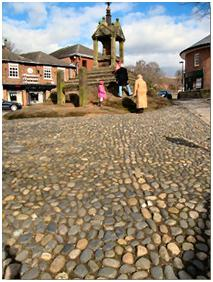
\includegraphics[width=0.5\textwidth]{TPA.jpg}
\caption[Cobblestone street in Lymm Cross, Cheshire, England]{Cobblestone street in Lymm Cross, Cheshire, England}\label{fig:TPA}
\end{figure}

\paragraph{Setts and Bricks} Setts are quarried stone blocks that are flat-topped (in contrast with round-topped cobblestones). They are typically arranged in a uniform matter, as pictured in \figref{TPBC}. Bricks are used and placed in a similar nature, but come from a different source material.  The road texture of sett-paved roads can vary depending on the evenness of the selected setts \cite{TP4}.

\begin{figure}[h]
\centering
	\begin{subfigure}[t]{0.4\textwidth}
		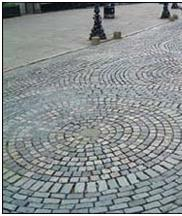
\includegraphics[width=\textwidth]{TPB.jpg}
	\end{subfigure}
	\begin{subfigure}[t]{0.4\textwidth}
		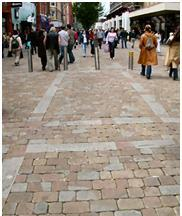
\includegraphics[width=\textwidth]{TPC.jpg}
	\end{subfigure}
\caption{Streets paved with setts}\label{fig:TPBC}
\end{figure}



\begin{figure}[h]
\centering
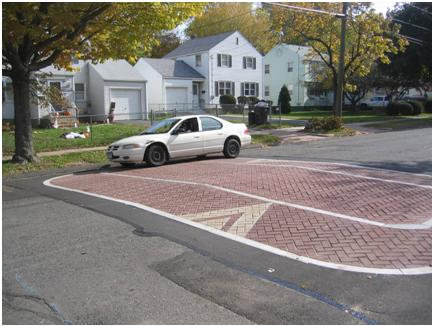
\includegraphics[width=0.5\textwidth]{TPD.jpg}
\caption[Speed hump utilizing brick paving]{Speed hump utilizing brick paving}\label{fig:TPD}
\end{figure}

\paragraph{Concrete Blocks} Concrete blocks are pre-cast, individual blocks of concrete that are placed similarly to bricks or setts. An advantage of using concrete blocks is that they can be shaped and colored in different ways to create a desired appearance. For example, concrete blocks can be made to look like setts and bricks by casting them in a certain size and applying the proper coloring. An additional advantage of concrete blocks is their reduced cost \cite{TP5}.

\begin{figure}[h]
\centering
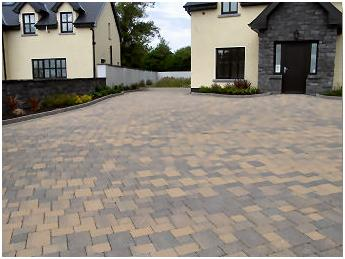
\includegraphics[width=0.5\textwidth]{TPE.jpg}
\caption[Concrete block paving]{Concrete block paving}\label{fig:TPE}
\end{figure}

\paragraph{Colored Pavement}Pavement can be colored through the use of pavement striping paint, as similarly used to make normal pavement markings. While textured pavements generally are made up of more earthen tones, bright colors can be used to create a very noticeable visual effect, as demonstrated by the green bike lanes in \figref{TPF}.

\begin{figure}[h]
\centering
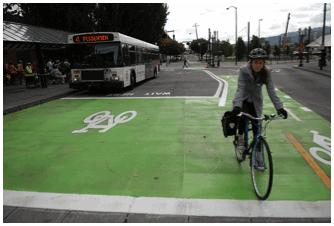
\includegraphics[width=0.5\textwidth]{TPF.jpg}
\caption[Green-colored bike lanes in Portland]{Green-colored bike lanes in Portland}\label{fig:TPF}
\end{figure}


\begin{figure}[h]
\centering
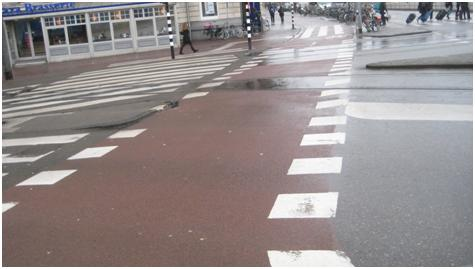
\includegraphics[width=0.5\textwidth]{TPG.jpg}
\caption[Brown coloring used to distinguish a bike path crossing in the Netherlands]{Brown coloring used to distinguish a bike path crossing in the Netherlands}\label{fig:TPG}
\end{figure}

\subsubsection{Cost}

The cost of utilizing textured or color pavements is dependent on a) the material used and b) the total area of the pavement. The Victoria Transport Policy Institute estimates a cost range of \$5--\$16 per square foot \cite{TP3}. A crosswalk 10 feet in width crossing a four-lane road, for example, would have a total material cost ranging from \$2400--\$7680.

	\subsection{Dignified Zones}
		\todo[inline]{Jake: Add the dignified zones section}
		Pedestrian & Restricted Traffic Zones

A pedestrian zone is an urban area in which motorized vehicle access is disallowed. In some instances, all wheeled vehicles (including bicycles) are banned from the zone. Barriers are typically put in place to physically obstruct motorized vehicles from entering. These barriers typically come in the form of bollards (pictured below) and can be either permanent or removable, if access is required for certain motorized vehicles. Pedestrian zones can be created temporarily by closing off a normal street to motorized traffic by placing temporary barriers. Alternatively, permanent pedestrian zones can be designed without motorized traffic in mind. \figref{PZA}, \figref{PZC}, and \figref{PZD} illustrate examples of permanent pedestrian zones \cite{PZ4}.
 
\begin{figure}[h]
\centering
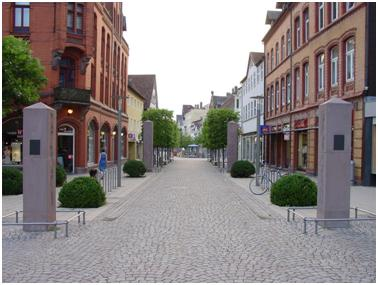
\includegraphics[width=\textwidth]{PZA.JPG}
\caption[Example of pedestrian zone design]{Example of pedestrian zone design: enough space allowed in the middle for essential motor vehicles, textured pavements to indicate an alternative purpose for the space, and bike racks in place to encourage bicycle use.}\label{fig:PZA}
\end{figure}

\begin{figure}[h]
\centering
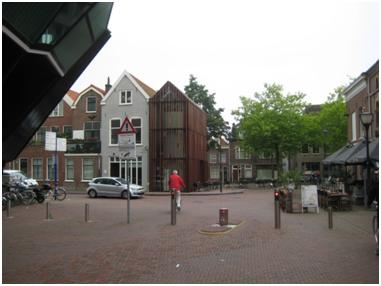
\includegraphics[width=\textwidth]{PZB.JPG}
\caption[Bollards restricting access to a pedestrian area]{Bollards restricting access to a pedestrian area}\label{fig:PZB}
\end{figure}

\begin{figure}[h]
\centering
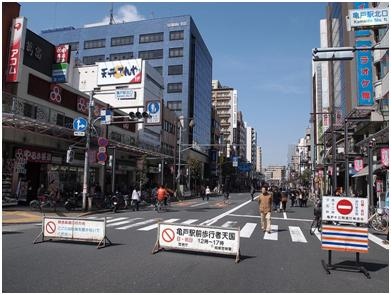
\includegraphics[width=\textwidth]{PZC.JPG}
\caption[A temporary pedestrian zone in Tokyo]{A temporary pedestrian zone in Tokyo, created by placing temporary barriers in front of a normal street}\label{fig:PZC}
\end{figure}

Pedestrians zones make land that was previously used for roads or parking available for gathering space or green space. Pedestrian zones increase the local populationís use of walking as a mode of transportation, which in turn decreases usage of automobiles, as businesses in the zone have increased their accessibility to pedestrians. Additionally, these zones are also known to increase rates of physical activity, particularly amongst children \cite{PZ4}.
 
\begin{figure}[h]
\centering
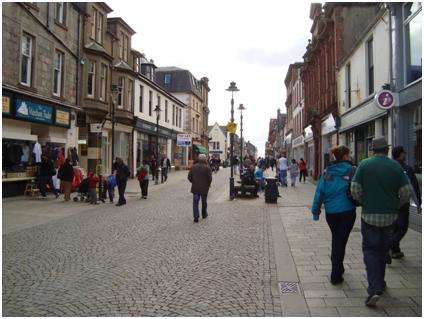
\includegraphics[width=\textwidth]{PZD.JPG}
\caption[A pedestrian zone]{A pedestrian zone}\label{fig:PZD}
\end{figure}

Restricted Traffic Zones are urban areas where non-essential motorized traffic is disallowed. This is a practice most commonly found in Italy, know as a \emph{zona traffico limatato}. The practice is used to reduce congestion and pollution in historical city centers. Cameras are placed at strategic checkpoints entering the zone to check control access. A picture is taken of every vehicle, and its license plate is cross-referenced against a list of permitted vehicles. Prohibited vehicles are fined. Depending on the characteristic of the restricted zone, other vehicles can be allowed as well, such as merchant vehicles, taxis, emergency vehicles, maintenance vehicles, and diplomats \cite{PZ1}. In combination with the closure of these zones to non-essential traffic, Italian cities increased public transit services to improve mobility. In Milan, for example, this practice proved to reduce automobile traffic in the zone by 50%. In Freiburg, Germany, traffic restriction and public transit improvements caused bicycle usage to double from 1976 to 1986 and led 18% of drivers to switch to public transit \cite{PZ2}. 
 
\begin{figure}[h]
\centering
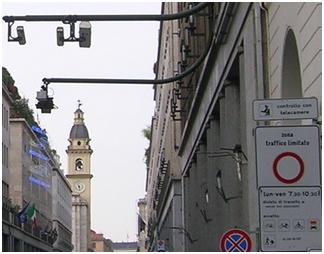
\includegraphics[width=\textwidth]{PZE.JPG}
\caption[\emph{Zona traffico limatato} warning sign and accompanying cameras]{\emph{Zona traffico limatato} warning sign and accompanying cameras}\label{fig:PZE}
\end{figure}

Costs

The primary costs of a restricted traffic zone are the construction and maintenance of the monitoring equipment; however, the fines (starting at an equivalent of $50 in Italy) collected due to violations would make up the difference \cite{PZ1}. One problem with these fines is that it is a nuisance to unsuspecting tourists who are not aware of the laws and fines. Additionally, if measures arenít taken to reduce total automobile traffic through public transit improvements, the traffic that is redirected due to these restrictions could cause significant congestion in other city zones.

The cost of introducing a pedestrian zone to an urban area depends on its design. Table A lists selected pedestrian improvements that could potentially be implemented in a pedestrian zone, and their estimated costs based on data from the San Francisco Bay Areaís Metropolitan Transportation Commission \cite{PZ8}.

[TABLE HERE NAKUL] Table A. Cost estimates of various elements of pedestrian zones \cite{PZ3}.
 
Total maintenance costs would also be dependent on the particular facilities. For an example of these costs, one can look to Corona Plaza in New York City. This proposed plaza is currently a dilapidated access road and parking lot, and is planned to be converted to a 13,000 square foot pedestrian public space \cite{PZ10}. It is estimated that it will cost between $50,000 and $75,000 a year to maintain this plaza \cite{PZ11}.

	\subsection{Traffic Circles}
		\todo[inline]{John: Add the traffic circles section}
		A traffic circle is a type of circular intersection.  It contains a center island, around which traffic flows in one direction.  A traffic circle can have one or multiple lanes inside of it, concentric about its center island.  Also referred to as a rotary or roundabout, it is capable of handling multiple street inputs.  They are commonly utilized throughout New England and Europe.

\begin{figure}[!htbp]
\centering
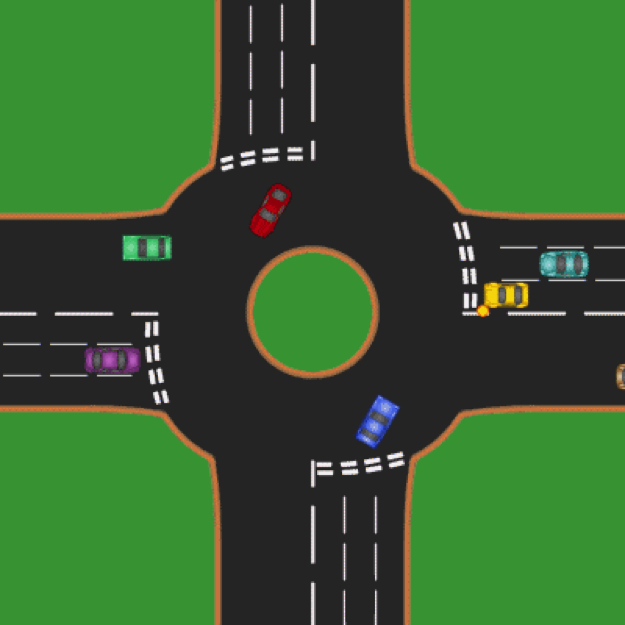
\includegraphics[width=0.5\textwidth]{roundabout}
\caption{A typical traffic circle for a four way intersection\cite{rabout1}}\label{fig:roundabout}
\end{figure}

Unlike a traditional intersection between two perpendicular streets, traffic circles generally do not have traffic lights controlling the flow of traffic.  Rather, traffic is controlled by right of way rules.  Typically, cars already in the traffic circle have right of way over cars seeking to enter into the traffic circle \cite{rabout2}.  Thus, they are designed to slow traffic.  Entering traffic typically yields to traffic already in the rotary, and allows for continuous flow of traffic to multiple exits.

Roads can enter a traffic circle radially or tangentially. Roads that enter radially require slowing down of speed and making a turn, thus acting as a traffic calming measure.  Roads that enter tangentially do not require as much reduction in speed or turn angle, so traffic is not slowed down as much \cite{rabout3}.  Though not as common, entry into traffic circles can also be regulated by traffic lights or stop signs.  

Another advantage of roundabouts is that they allow for easy exit to any of the roadways that connect to it.  With a normal perpendicular intersection, vehicles wanting to make left or right hand turns instead of continuing straight must wait for specific light signals to turn onto the desire road.  With a roundabout, a vehicle simply stays in the traffic circle until reaching its desired exit, which even allows for legal u-turns \cite{rabout1}.

\begin{figure}[!htbp]
\centering
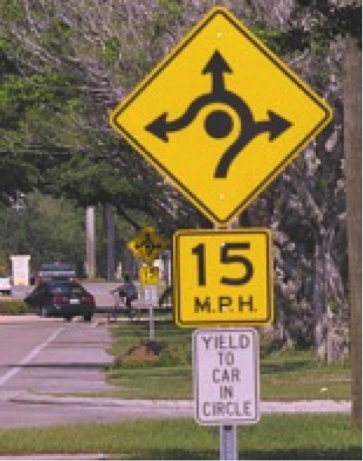
\includegraphics[width=0.5\textwidth]{roundabout-signage}
\caption[Roundabout Signage]{Entering traffic must slow and yield to vehicles already in the circle}\label{fig:roundabout-signage}
\end{figure}

\subsubsection{Advantages and Disadvantages}
The advantages of roundabouts are:\begin{itemize}
	\item Eliminates T-bone (perpendicular) crashes and head on collisions
	\item Allows for continuous entering and exiting of traffic to any street
	\item Improved flow over traffic lights
	\item Calms traffic by reducing speed without complete stops
\end{itemize}

Roundabouts come with the following drawbacks:\begin{itemize}
	\item Lacks computerized traffic control features
	\item Can become congested
	\item Not efficient at moving high volumes of vehicles
	\item Confusing for inexperienced drivers
	\item Require driver decision making and timing
\end{itemize}

\subsubsection{Capacity}
The capacity of a roundabout is dependent upon the number of lanes within the circle, as well as the diameter of the circle.  Most modern roundabouts are less than 250 feet in diameter \cite{rabout1}.  Since it does not necessarily require a full stop by entering vehicles, traffic circles can provide less delay than light controlled intersections.  When the volume of entering traffic is unequal between the different roads (unbalanced), there can be inefficiencies.  Traffic lights are optimized to maximize the traffic throughput by giving more green lights to a busier road, whereas with a roundabout all roads must slow down and yield to traffic within the roundabout, regardless of the amount of traffic on any particular road \cite{rabout4}.  On the other hand, when all of the entering roads experience constant and balanced traffic, a traffic circle can reduce wait times by eliminating red lights.  

\begin{figure}[!htbp]
\centering
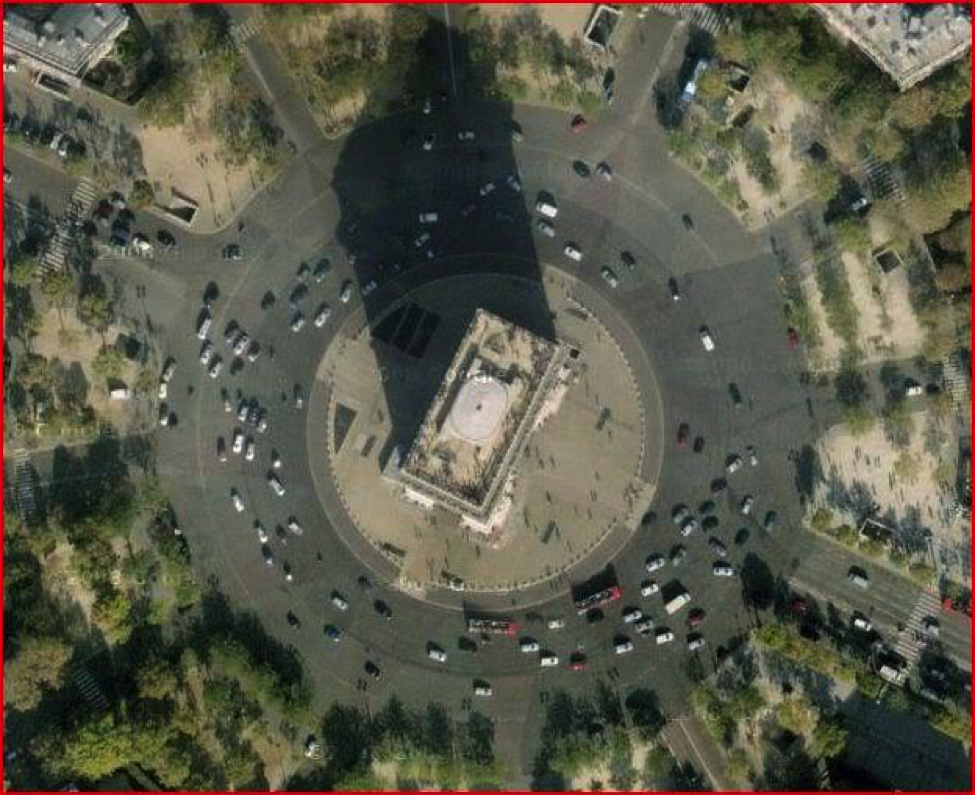
\includegraphics[width=0.5\textwidth]{arc-de}
\caption[Place de l'Etoile]{Perhaps the most well-known traffic circle is the Place de l'Etoile around the Arc de Triomphe in Paris, which has eight lanes with twelve avenues feeding into it.}\label{fig:arc-de}
\end{figure}

\clearpage

\subsubsection{Mini-roundabouts}
One specific type of traffic circle is a mini-roundabout.  Mini-roundabouts can be built in places where there is not enough space for a traditional roundabout.  They are used in place of a four way stop or traffic light controlled intersection.  They improve efficiency by eliminating the delay caused by stop signs and traffic signals.

\begin{figure}[!htbp]
\centering
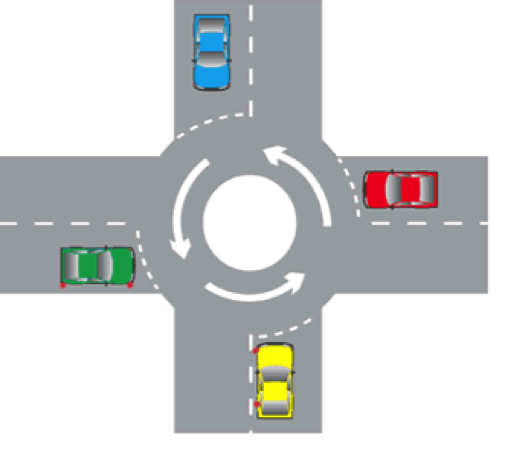
\includegraphics[width=0.5\textwidth]{mini-rabout}
\caption[Mini-Roundabout]{Mini-roundabouts offer greater efficiency than stop signs or lights for intersections with single lane roads.}\label{fig:mini-rabout}
\end{figure}

	\subsection{Midblock Crossings}
		\todo[inline]{John: Add the midblock crossings section}
		Midblock crossings are crosswalks that are located on streets in places other than intersections.  They are a safer alternative to pedestrians jaywalking at unmarked points.  Most crosswalks are located at intersections, where traffic lights allow for vehicles to be controlled in order for pedestrians to safely cross the street.  In dense, urban locations with short blocks, this works well.  However, in areas with long stretches of road between intersections, it is not always convenient to have to cross at an intersection.  Many pedestrians will jaywalk across a street at the location where they need to cross it, not necessarily at an intersection.  This can present a hazard to both pedestrians and vehicles, as they could cross the street at any point, and approaching vehicles may not be able to see them.  One study shows that midblock jaywalking was responsible for 26.5\% of all pedestrian accidents \cite{mid1}.

With long blocks, long signals, wide intersections, and high vehicle speeds, crossing at intersections isn’t always easy.  It becomes important to identify points at which it is practical and safe to cross roads.  Without them, pedestrians make their own decisions to cross at random points, creating risk for both themselves and drivers.  By increasing the number of midblock crossings, we hope to decrease the occurrence of jaywalking while improving pedestrian mobility.

\begin{figure}[!htbp]
\centering
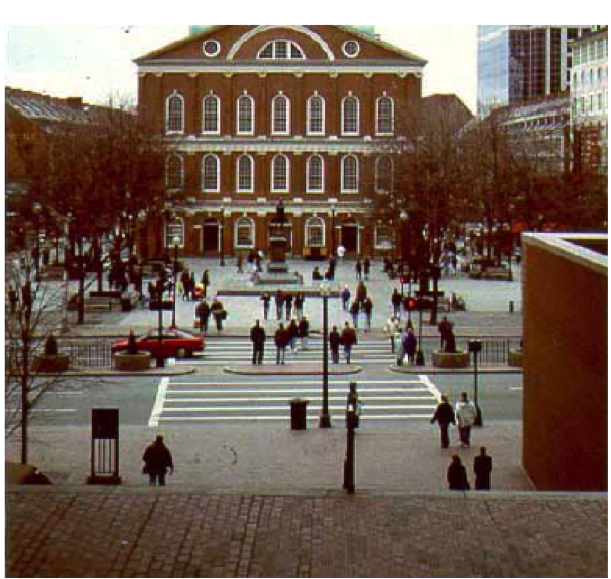
\includegraphics[width=0.5\textwidth]{midblock}
\caption[Midblock Crossing]{Midblock crossings safely connect public places between intersections.}\label{fig:midblock}
\end{figure}

\subsubsection{Medians}
Medians, also called refuge islands, are often necessary for high volume and high speed roads.  Without them, crosswalks are simply too long to cross.  They provide a convenient resting area halfway through a crosswalk where pedestrians can safely wait until the other lanes of traffic are safe to cross.  It can be difficult to find a suitable gap in traffic for multiple lanes, with traffic heading in both directions.  A median can cut the number of lanes in half by creating two separate crossing journeys, each with traffic in only one direction \cite{mid2}. 

For low volume and low speed roads, medians often are not necessary.  Gaps in traffic are easier to navigate, and the walking distance across the crosswalk is shorter.  For roads with traffic above 30 mph and high traffic volume, midblock crossings should utilize signals and other control devices \cite{mid2}.

\begin{figure}[!htbp]
\centering
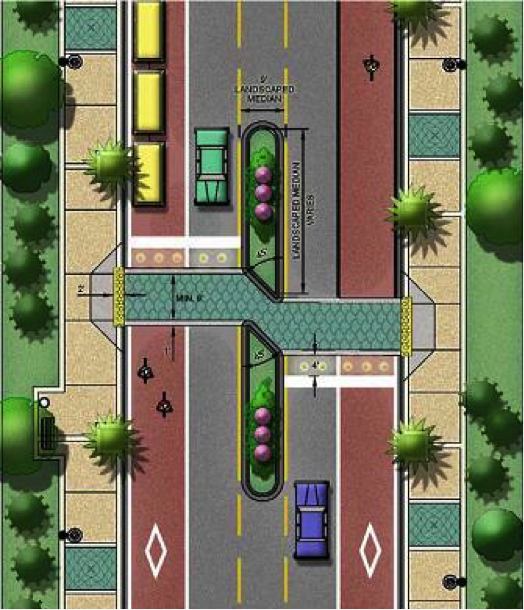
\includegraphics[width=0.5\textwidth]{median}
\caption[Median]{Medians divide long crosswalks into two shorter ones.}\label{fig:median}
\end{figure}

\section{Analysis}
	\subsection{Methodology}
		\todo[inline]{Jake: Talk about the methodology we used}
		As part of scope of this project, this group has been charged with ranking the previously spotlighted best practices. The purpose of this ranking system is to concretely define which practices, in the opinion of this group, would be most recommended for implementation into the Mobility Element of the city's General Plan as important street design principles.

The Victoria Transport Policy institute lays out a framework for evaluating traffic calming practices. They identify four factors that influence the effectiveness of a particular project:\begin{description}
	\item[Magnitude of Change] How much of an influence a particular measure has on improving pedestrian and cyclist mobility.
	\item[Demand] Improvements to streets are more effective if more people utilize them.  For example, pedestrian facility improvements should be made around busier areas such as schools or commercial centers \cite{TP3}.
	\item[Integration with other improvements]  If only one complete street design practice is applied in an improvement project, it has much less of impact than if many other practices were applied in the same project \cite{TP3}.
	\item[Land use effects] Street improvements that promote pedestrianism can cause changes in land use that further encourage people to walk or cycle, such as shops spring up along busy pedestrian corridors \cite{TP3}.
\end{description}

Since the best practices that have been outlined previously are being examined as general practices, rather than as improvements to specific locations, they will be evaluated based on their individual magnitudes of change, how well they integrate with other practices, and the feasibility of implementing them in the context of Los Angeles. 

To determine each practice's usability index, a score has been assigned to each practice for four characteristics: magnitude of change, integration with other improvements, viability in Los Angeles, and cost. Each practice is rated `low', `medium', or `high'. These scores are derived from the judgment of group members in combination with ratings of a similar nature from San Francisco's Metropolitan Transportation Commission \cite{PZ7}. The Usability Index score is an agglomeration of these four scores, also with ratings of low', `medium', or `high'.
	\subsection{Rankings}
		\todo[inline]{Jake: Rank the practices}
		
% Booktabs require to add \usepackage{booktabs} to your document preamble
\begin{table}[h]
\begin{tabular}{@{}llllll@{}}
\toprule
Practice                                                                & \begin{tabular}[c]{@{}c@{}}Magnitude of\\ Change\end{tabular} & \begin{tabular}[c]{@{}c@{}}Integration with\\ other improvements\end{tabular} & \begin{tabular}[c]{@{}c@{}}Viability in\\ Los Angeles\end{tabular} & Cost   & \begin{tabular}[c]{@{}c@{}}Usability\\ Index\end{tabular} \\ \midrule
Chokers                                                                 & Medium                                                        & Medium                                                                        & High                                                               & Medium & High                                                      \\
Curve Radii                                                             & Medium                                                        & High                                                                          & High                                                               & Medium & High                                                      \\
Raised Crosswalks                                                       & Low                                                           & Medium                                                                        & Medium                                                             & Medium & Medium                                                    \\
Curb Extensions                                                         & Medium                                                        & High                                                                          & High                                                               & Medium & High                                                      \\
\begin{tabular}[c]{@{}c@{}}Textured \& Colored\\ Pavements\end{tabular} & Low                                                           & High                                                                          & High                                                               & Low    & Low                                                      \\
Pedestrian Zones                                                        & High                                                          & High                                                                          & Low                                                                & High   & High                                                      \\
Traffic Circles                                                         & Medium                                                        & Low                                                                           & Medium                                                             & Medium & Medium                                                    \\
Midblock Crossings                                                      & Medium                                                        & Low                                                                           & High                                                               & Medium & Medium         \\
\bottomrule                                          
\end{tabular}
\caption{Rankings of Best Practices}
\end{table}
	\subsection{Discussion}
		\todo[inline]{Jake: Discuss the results}
		Upon reflection, select individual ratings stand out, specifically, the `low' rating of pedestrian zones for viability in Los Angeles. The group felt that one particular challenge with implementing pedestrian zones was that in most examples, they were typically put in place in areas with high population density. In the context of Los Angeles, and specifically South Los Angeles, the group felt that it would be difficult to select a location for a pedestrian zone, and that pedestrian traffic should instead first be built up in such a manner that a pedestrian zone would be more accessible when it is finally implemented. That said, the group ultimately rated pedestrian zones with `high' usability index due to the significant benefits they can provide to public health.

Research into the subject found there is no consensus on the ability of textured or colored pavements to reduce vehicle speeds, which significantly contributed to its `low' usability index rating; however, most examples of textured pavement found by the group were in combination with other street elements, such as raised crosswalks, traffic circles, or pedestrian zones. The visual cue that textured and colored pavements provide to drivers and pedestrians, combined with potential aesthetic benefits, make them good accents for other projects, but not viable as a standalone improvement. 

In addition to the previously discussed pedestrian zones, the group finds chokers, curve radii, and curb extensions to be of high usability to the city. The commonality between these practices is that they contribute to mobility by creating safer environments for pedestrians, and are extremely viable in a city such as Los Angeles, where there are numerous available location for these practices to be implemented.

\section{Conclusion}
	A city's choice of guiding principles behind street design has a large impact on the daily life of its people. This is especially true in an area like Los Angeles, where so many depend on the ubiquitous roads to get between home, work, and school. Thus, it is important that decisions with regard to policy must be made keeping in mind the needs of all parties involved: commuters, pedestrians, residents, and local business owners.

The research that we have done into the `best practices' currently in use at various locations around the world has revealed telling data on the effects these measures have had on their neighborhoods. The existence of these quantified metrics allowed us to evaluate these practices in an objective manner, and determine which practices would be appropriate for the Los Angeles area.

We hope that our findings will assist the CHC with selecting and promoting better mobility policies. Should these be succesfully petitioned to our policymakers, they will translate into streets that are safer and cleaner.
	\todo[inline]{Nakul: Conclude}

%description, impact, cost

\newpage

\nocite{*}
\bibliography{citations}{}
\bibliographystyle{plain}

\newpage

\todo[inline]{Jake: Add your resume to the resumes subfolder}
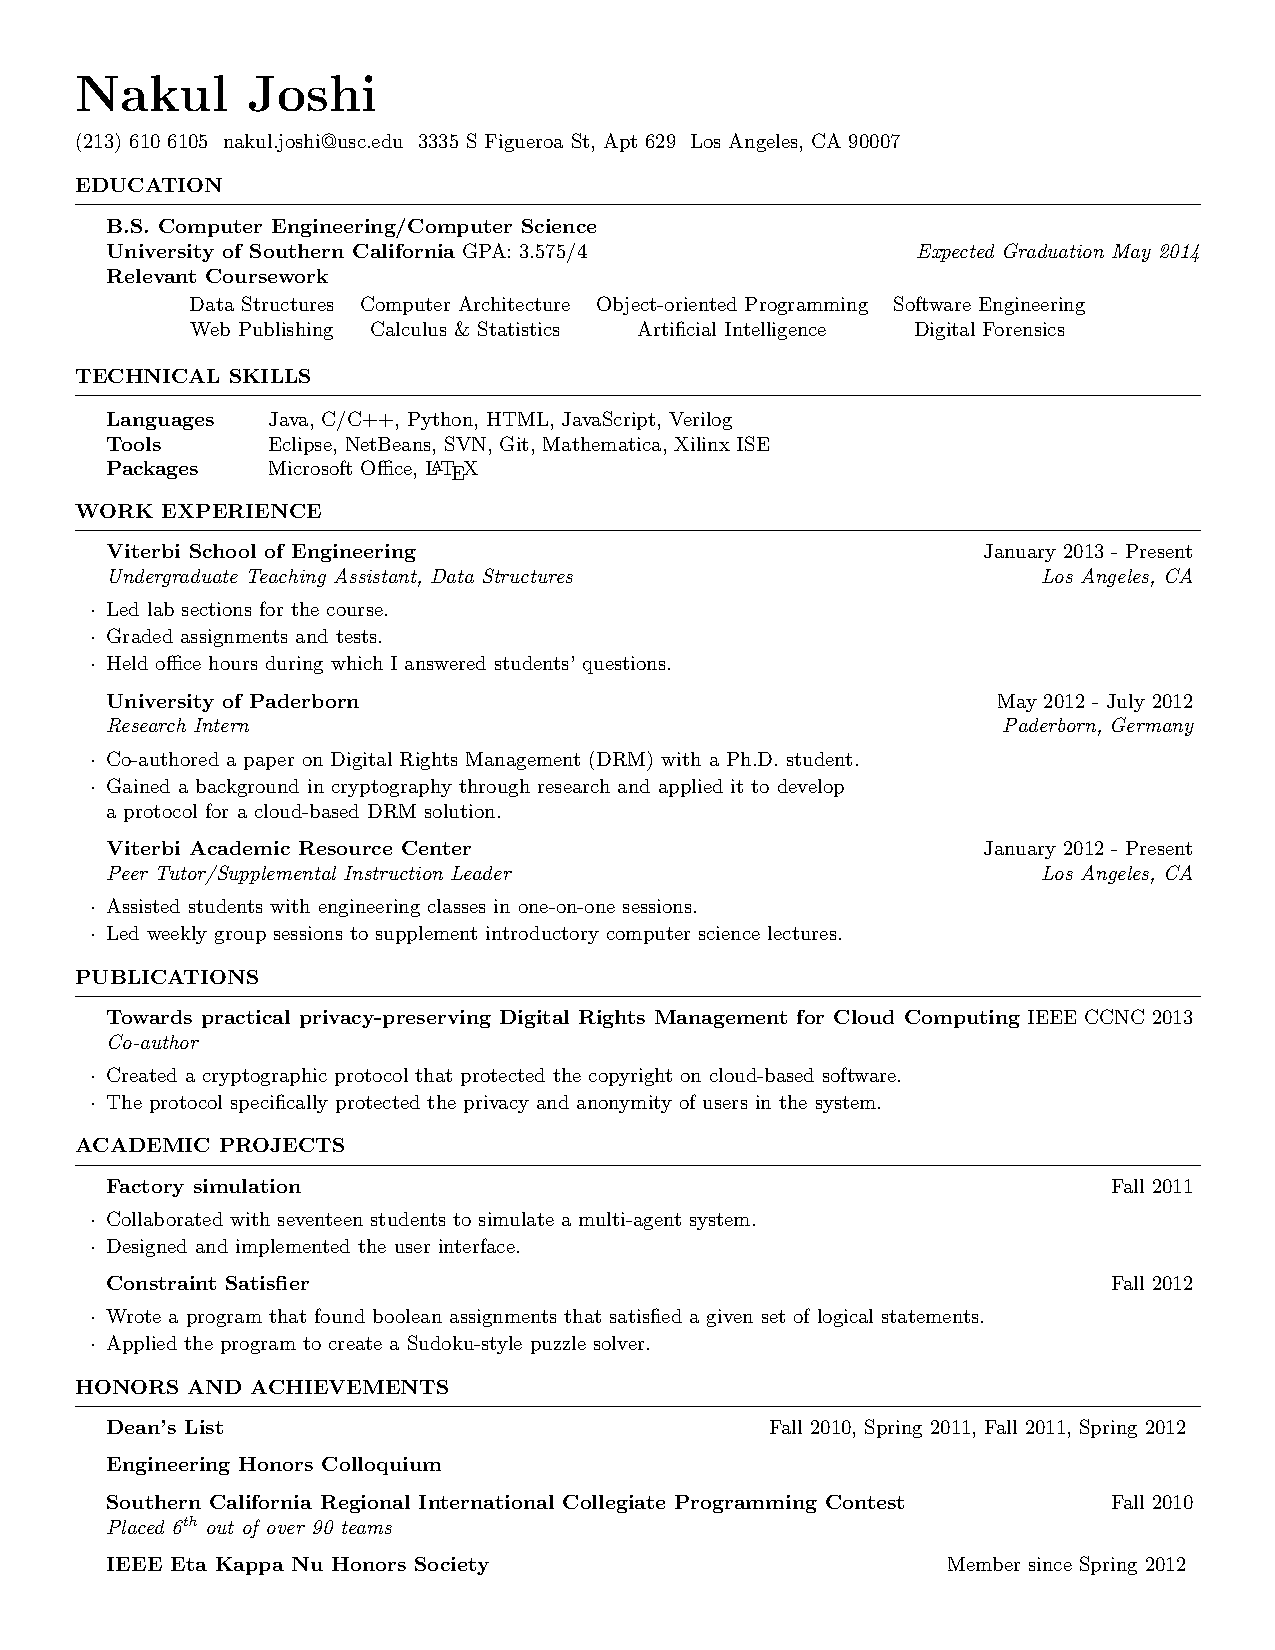
\includepdf{resumes/nakul.pdf}
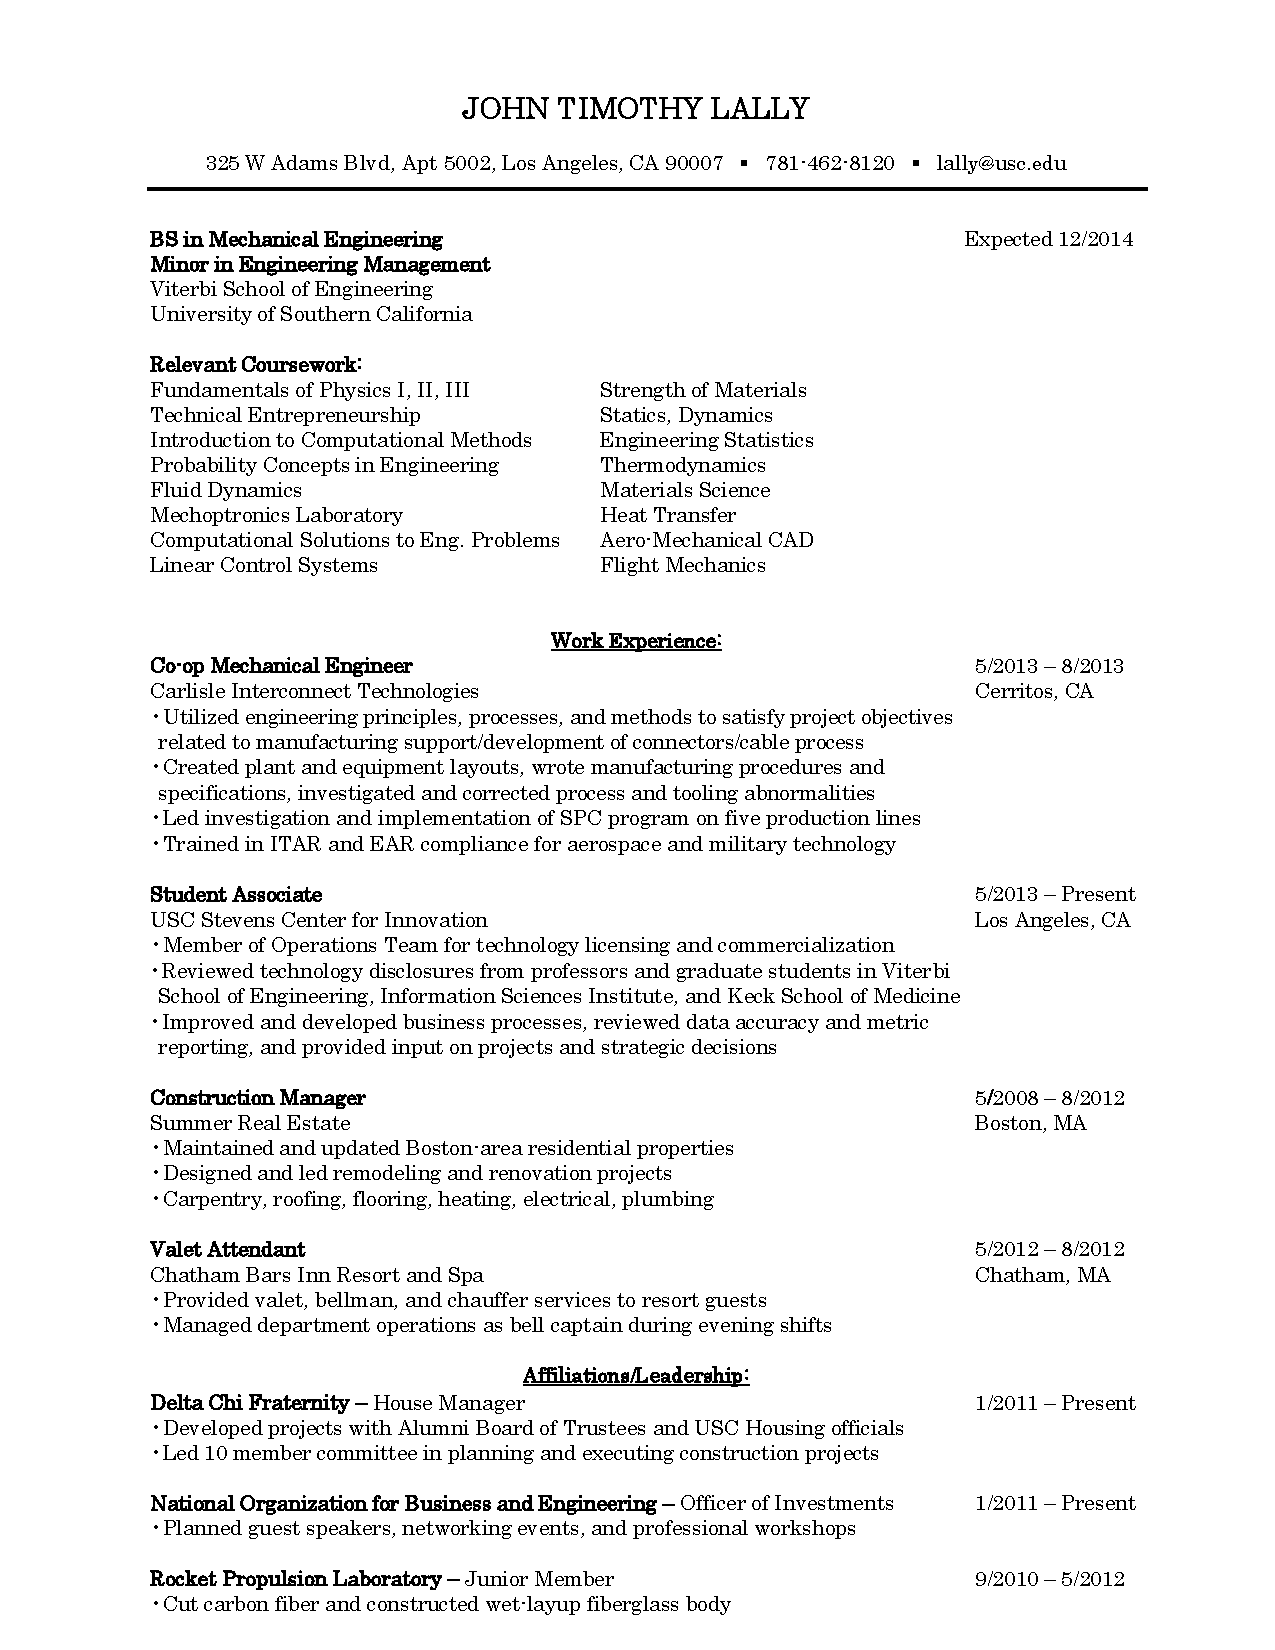
\includepdf{resumes/john.pdf}

\includepdf{resumes/christine.pdf}


\end{document}